\chapter{The Reactive Component Model \label{model}}

\paragraph{Overview.}
In this chapter, we present a model for composing and decomposing reactive programs called \emph{reactive components}.
The model is biased toward practical software development even as it enforces properties based in formal methods.
Consequently, the model favors utility, practicality, flexibility, and ease of implementation.

%% \paragraph{Formal models and software engineering.}
%% I claim that most of the software that is ``put into production'' will never be proved formally correct.
%% This is a function of economics since modeling and constructing proofs is a labor-intensive process that can only be justified for safety or mission critical software.
%% However, I would argue that the development and application of formal models are critical to software engineering.
%% To illustrate, consider \emph{structured programming}~\cite{dahl1972structured}.
%% Structured programming assumes an abstract machine that executes programs that are restricted to a small set of well-defined control structures and assignment statements.
%% A program written in this form can be reasoned about directly from the text by formulating a Hoare-triple for each statement.
%% Structured programming opened the door for \emph{structured programming languages} which are also based on well-defined control structures and evaluation semantics.
%% Thus, while very few programmers will prove their structured programs correct, all of them informally use structured programming when they are fixing a bug revealed by a unit test or analyzing a core dump in a debugger.
%% Structured programming languages reduced the accidental complexity associated with writing the same program in assembly language.

%% The realm of reactive programs is waiting for a similar reduction in accidental complexity.
%% Taking a hint from structured programming, I believe two things are required.
%% First, we must write reactive programs against an easy-to-reason-about abstract machine instead of low-level interfaces like atomic instructions and thread libraries.
%% Second, we must restrict the form of reactive programs so that they can be reasoned about from the text.
%% I hope the proposed model of reactive systems is a step toward toward this goal.

\begin{figure}
\centering
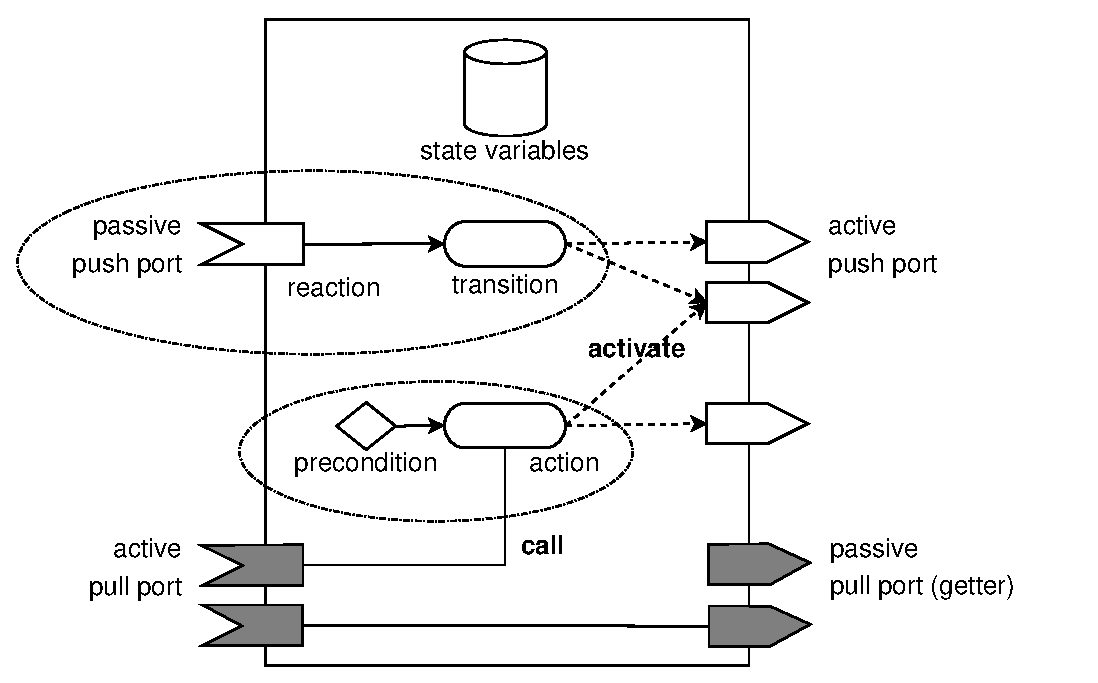
\includegraphics[width=\textwidth]{reactive_component.eps}
\caption{Diagram depicting the features of a reactive component\label{reactive_component}}
\end{figure}

Figure~\ref{reactive_component} shows the major features of a reactive component.
Like other state-based formal models, the core of a reactive component is a set of \emph{state variables} and a set of atomic \emph{transitions} that manipulate those state variables.
When reasoning about a system, behavior is expressed as propositions over the state variables where the propositions are derived from the transitions.
The contribution that this work makes to existing state-based formal models of reactive systems is a number of interface elements and composition semantics that allow reactive programs to be composed in a principled way.
For example, an \emph{active push port} allows a transition in one component to be linked to a transition in another component such that the resulting transaction is atomic.
Active push ports allow reactive components to publicize their behavior.
An active push port may be \emph{bound} to and conditionally \emph{activate} zero or more \emph{passive push ports}.
A passive push port names the corresponding transition that will be executed when the passive push port is activated.
This combination of passive push port and transition is called a \emph{reaction} because it reacts to a transition in another component.
The atomic linkage of a transition in one component to a transition in another component through the push port mechanism allows the properties of each component to be related to one another and complex systems to be constructed by composing simpler systems.
Transitions that are not executed via a passive push port have a precondition that nominates them for execution by a weakly fair scheduler.
The combination of a precondition and transition is called an \emph{action} because it is a voluntary transition under the control the containing component.
An \emph{active pull port} represents an immutable external data dependency.
The component may \emph{call} an active pull port to yield a value required in a transition.
Active pull ports must be bound to a \emph{passive pull port} which resembles a function returning a value, e.g., a getter or a predicate.
Where push ports allow components to publicize their behavior, pull ports allow components to safely publicize their internal state for use by other components.

Composition in the reactive component model has two main features.
The first is recursive encapsulation where a state variable in one component may represent an instance of another reactive component.
The second is the ability to bind push ports and pull ports through an \emph{explicit} set of \emph{bindings}.
The decision to use an explicit set of bindings as opposed to implicit named-based matching is more inline with the goals and techniques of practical software development since it facilitates the use of software developed under different naming conventions, i.e., third-party software.
A third minor feature called \emph{exporting} is the ability of an encapsulating component to adopt interface elements of its sub-components without defining complimentary ports and transitions that do nothing but forward an activation or call.
The ability to publicize behavior and state and the ability to assemble well-defined behavior from existing behaviors in a straight-forward and flexible way are the defining characteristics of the reactive component model.

\begin{figure}
\centering
\includegraphics[width=\textwidth]{web_server.eps}
\caption{Diagram of a web application built using reactive components\label{web_server}}
\end{figure}

To illustrate the utility of component interfaces and composition, we present a design for a web application or web server using reactive components in figure~\ref{web_server}.
The web application consists of five reactive components.
The first is an unnamed top-level component representing the complete application.
This component has four sub-components representing a web server, the application logic, a database, and a logging service.
The ports of the application logic have been bound to the corresponding ports in the web server, database, and logging service.
The interface of a component, which consists of its ports, provides insight into the behavior of a component.
For example, by just inspecting the interface of the web server component we expect it to 1) verify incoming HTTP requests with the application\footnote{A production web server may verify that the requested HTTP method can be applied to the given URI, that content length limits are respected, that content types are supported, etc.}, 2) pass on valid HTTP requests to the application, and 3) send HTTP responses to the web client.

Figure~\ref{web_server} also demonstrates how reactive programs can be constructed by composing reactive components.
From a software engineering perspective, it behooves a developer to focus on the application logic and use already developed components for the web server, database, and logging service.
Furthermore, one can imagine developing three stateless components surrounding the application logic that do nothing but translate messages to and from application specific message types to the generic types required by the web server, database, and logging service.
The application logic, then, is completely isolated from the surrounding libraries and may be tested by providing mock components for the web server, database, and logging service.
The application logic itself has a well-defined interface and could be reused, say, by implementing a graphic front-end to drive the application instead of a web service.

%% \begin{figure}
%% \centering
%% \includegraphics{composition.eps}
%% \caption{Diagram of a component consisting of four sub-components\label{composition}}
%% \end{figure}

%% Figure~\ref{composition} shows a reactive component consisting of four sub-components labeled A, B, C, and D.
%% Internals elements, i.e., the state variables and transitions, have been elided for clarity.
%% The solid lines connecting ports are \emph{bindings} that explicitly link active push ports to passive push ports and active pull ports to passive pull ports.
%% The interface of the top-level component consists of a single active push port that \emph{exports} the active push port of component B.
%% From figure~\ref{composition}, we know nothing about the state variables and transitions of the components so we cannot describe in detail the properties of the top-level component.
%% However, from the diagram, we can conclude that component C is an internal ``sink'' and doesn't contribute the visible behavior of the top-level component.
%% Furthermore, we can conclude that

%% \paragraph{Reactive components and instances.}
%% A \emph{reactive component} is an abstract data type consisting of a set of \emph{state variables} and a set of associated \emph{atomic state transitions} \emph{TODO}.
%% An \emph{instance} of a reactive component is a physical realization \emph{TODO} of a reactive component.
%% By analogy, reactive components and instances correspond to classes and objects, respectively, in object-oriented programming.
%% This is a departure from formal models like UNITY and I/O Automata where one reasons directly with instances.
%% The main reason for this departure is that it facilitates a straight-forward implementation of the model in a strongly-typed programming language.
%% This dissertation uses the general term \emph{reactive component} when a distinction between type and instance is irrelevant or obvious from context.
%% When such a distinction is important, this dissertation uses \emph{reactive component type} or \emph{reactive component instance}.

\paragraph{State variables.}
Half of the internal core of a reactive component is a set of state variables.
When modeling, the state variables are subject of the various propositions that demonstrate the behavior of the system.
When implementing, the state variables are manipulated by the various assignment statements that constitute the transitions.
As in other formal models, the types of the state variables may be selected to make writing proofs easier.
That is, the types of state variables are mathematically friendly like integers, sets, and lists.
Implementations of the reactive component model must provide a type system that allows the state variables to be realized on the machine of interest.
The type of a state variable may be a reactive component type which facilitates recursive encapsulation.
For modeling purposes, state variables typically have \emph{value semantics} meaning we need not reason about references.
As a practical concession, however, we will introduce pointers for building arbitrary linked data structures since we advocate an imperative state-based implementation and describe the issues of introducing pointers into the reactive component model.

\paragraph{Atomic state transitions.}
The other half of the internal core of a reactive component is a set of atomic state transitions that manipulate the state variables.
A precise definition of the atomicity of state transitions will be deferred to the discussion on composition and execution.
State variables and state transitions are private meaning that transitions can only refer to the state variables of the associated reactive component and a transition in one reactive component can only be linked to a transition in another component through the composition mechanisms.
Thus, all initialization and updates to state variables can be determined by examining the transitions of the corresponding component.
This means that composition is \emph{compositional} meaning that a property established for a reactive component independent of context can never be violated since the set of transitions from which the properties were derived is fixed.
State transitions must be deterministic meaning that the next value of every state variable is uniquely and well defined.

The reactive component model does not prescribe a specific language for encoding state transitions.
The language used depends on the goals and tastes of the one developing or analyzing the model.
For example, expressing transitions using the programming language of UNITY~\cite{chandy1989parallel} may allow the modeler to extract proofs from the text, a major goal of UNITY.
The approach used by I/O Automata~\cite{nancy1996distributed} is to specify the condition established by each transition.
The approach used by the implementation presented in this dissertation uses a C-like language augmented for port activations to encode the state transitions.

%% For presentation, a state transition is represented by a multiple assignment statement akin to the multiple assignment statements in UNITY~\cite{chandy1989parallel}.
%% A transition is a list of assignment clauses: $clause_0 \; || \; ... \; || \; clause_n $.
%% Each clause is either an unconditional assignment or a conditional assignment\footnote{UNITY also includes a quantified assignment clause which can used without loss of continuity}.
%% An unconditional assignment has the form $LHS := RHS$ where $LHS$ is a list of lvalues and $RHS$ is a list of expressions.
%% A conditional assignment has the form $LHS := \mathrm{if} \; condition_0 \; \mathrm{then} \; RHS_0 \; \mathrm{else~if} \; ... \; \mathrm{else} \; RHS_n$.
%% In UNITY, the conditions are used as preconditions to guard the execution of the assignment statement.
%% However, in reactive components, the conditions are merely used to provide alternative values.
%% Consequently, the conditions in the conditional assignment must be disjoint and cover all of the cases so that the variables in $LHS$ are well-defined after the assignment is executed.
%% Conceptually, the $RHS$ represents the next values for the state variables on the $LHS$.
%% The arity of $LHS$ must be the same as $RHS$ and corresponding elements of $LHS$ and $RHS$ are type compatible.
%% For determinism, every element of $LHS$ must be unique\footnote{This is a departure from UNITY where state variables can be repeated on the LHS but must all have the same next value.}.

\paragraph{Actions, reactions, push ports, and composition.}
A state transition is either part of an action or reaction.
An \emph{action} is a state transition whose execution is under the control of the component to which it belongs.
The action is guarded by a \emph{precondition} that is guaranteed to be true when the action is executed.
%% Actions are represented by augmenting the state transition with an optional \emph{precondition}: $\{ \mathrm{if} \; (precondition) \} \; LHS := RHS$.
The precondition is a Boolean expression that determines if the action is \emph{enabled} or \emph{disabled}.
If the precondition is absent, it is assumed to be true.

A \emph{reaction} is a state transition whose execution is under the control of another action or reaction.
Thus, we require a mechanism for linking a reaction to an action or another reaction.
To do this, we introduce the notion of a \emph{push port}.
A push port is a typed interaction point consisting of an active side that conditionally \emph{activates} the port and provides arguments to the port and a passive side that \emph{reacts} to the port and may access the arguments provided by the active side.
The transition associated with a passive push port is executed atomically with the transition that activates the active push port.
%% We revise the definition of a component to include a set of active push ports and passive push ports where each port has a (unique) name and signature.
%% An action then has an optional set of active push ports: $\{ \mathrm{if} \; (precondition) \} \; LHS := RHS \; \{\mathrm{activates} \; ports \}$ where $ports$ is a list of unique port activations.
%% A \emph{port activation} has the form $port_0(arg_0, ..., arg_n) \; ... \; \mathrm{if} \; condition$ where each $arg$ is an expression providing the value of the argument.
%% A reaction is a state transition augmented with a passive push port and an optional set of port activations: $port(signature) \; LHS := RHS \; \{ \mathrm{activates } \; ports \}$.
%% The $RHS$ and activations of a reaction may reference the arguments of the push port.

\paragraph{Execution.}
As with UNITY~\cite{chandy1989parallel} and I/O Automata~\cite{nancy1996distributed}, we assume the existence of a weakly fair scheduler that \emph{selects} and \emph{executes} enabled instance/action pairs.
Selection is \emph{serial} meaning that one action is considered and therefore executed at a time.
Thus, each action is atomic with respect to all other actions.
Selection is also \emph{non-deterministic} meaning that the scheduler is free to select any instance/action pair according to weak fairness which is described below.
This falls in line with the common practice of modeling concurrency with non-deterministically scheduled atomic actions.

A \emph{trace} is the sequence of instance/action pairs executed by the scheduler.
Weak fairness says that all instance/action pairs are selected an infinite number of times in an infinite run of the system.
The key point is the difference between selections and execution.
To illustrate, consider a component consisting of a single Boolean flag $b$ that is initially false and three actions labeled $A$, $B_0$, and $B_1$.
Action $A$ is enabled when $b = false$ and sets $b$ to true.
Actions $B_0$ and $B_1$ are enabled when $b = true$ and set $b$ to false.
A trace for this component resembles $ABAB \ldots$ where $B$ represents either $B_0$ or $B_1$.
Thus, an infinite trace will contain an infinite number of $A$s.
However, the same trace may contain an infinite number of $B_0$s with no $B_1$s, an infinite number of $B_1$s with no $B_0$s, or some combination of $B_0$s and $B_1$s.
The extreme cases illustrate weak fairness.
Assume the trace contains no $B_1$s.
From this, we can conclude that the scheduler always selected $B_0$ when $b = false$, which occurred an infinite number of times.

When an action is executed it may conditionally activate various push ports.
If these ports are bound to reactions, the reactions will be executed, their push ports conditionally activated and so on.
We divide a state transition into two steps called the \emph{immutable step} and the \emph{mutable step}.
Logically, a transition assigns values to a set of state variables.
This can be modeled as a multiple assignment statement with a left-hand side (LHS) consisting of a list of state variables and a right-hand side (RHS) consisting of a list of expressions that provide the next value for the corresponding state variable.
The immutable step corresponds to the computation of the RHS in a state transition.
The mutable step corresponds to the update of the values on the LHS with the values on the RHS.
When transitions are linked with composition, we must relate the mutable and immutable step in a state transition to the mutable and immutable steps in all dependent state transitions.
Let $A$ be a transition and $B$ be a transition that depends on $A$.
Let $A_I$ be the immutable step of $A$, $A_M$ be the mutable step of $A$, $B_I$ be the immutable step of $B$, and $B_M$ be the mutable step of $B$.
For the sake of argument, assume that $A_I$ reads variables that are written in $B_M$ and that $B_I$ reads variables that are written in $A_M$.
We require that $A_I$ be evaluated before $A_M$, $B_I$ be evaluated before $B_M$, and $A_I$ be evaluated before $B_I$ since activation is conditional.
This leaves three possible sequences of steps:
\begin{itemize}
\item $A_I A_M B_I B_M$.  In this sequence, a variable is first updated in $A_M$ and then the updated value is read in $B_I$.  The issue with this interpretation is that it does not compose well.  Ideally, we would like to be able to rewrite the transition as a single transition consisting of a single immutable step and mutable step.
\item $A_I B_I A_M B_M$ and $A_I B_I B_M A_M$.  These sequences resolve the issue with the first sequence by providing a clear immutable step and mutable step.
\end{itemize}
Thus, with respect to composed state transitions, all immutable steps (which includes all push port activations) are performed before all mutable steps.

\paragraph{An example.}
To illustrate reactive components, we rewrite the \emph{Clock automaton} example in ~\cite{nancy1996distributed} using reactive components.
The Clock automaton consists of a free-running counter and flag used to implement a request-response protocol.
The Clock automaton is listed in figure~\ref{clock_component}.
The state variables are identified with \verb+var+ and their initial values are provided.
The component contains a reaction \verb+request+ for receiving requests to sample the current value of the counter.
The component also contains an active push port \verb+clock+ for communicating the sampled value of the counter.
The first action \verb+Tick+ is an action that increments the free-running counter.
The absence of a precondition means this action is always enabled.
The second action \verb+Clock+ is conditioned on the flag variable (which indicates that a request has been made) which resets the flag and communicates the value of \verb+counter+ by activating the \verb+clock+ port.
A simple client for the Clock component that perpetually samples the clock is shown in figure~\ref{client_component}.

\begin{figure}
\begin{verbatim}
component Clock {
  var int counter (0)
  var bool flag (false)
  push clock(int t)

  Tick: counter := counter + 1

  reaction request() flag := true

  Clock: flag -> flag := false activates clock(counter)
}
\end{verbatim}
\caption{Definition of the Clock component\label{clock_component}}
\end{figure}

\begin{figure}
\begin{verbatim}
component Client {
  var bool flag (false)
  push request()

  Request: !flag -> flag := true activates request()

  reaction clock(int t) flag := false || /* do something with t */
}
\end{verbatim}
\caption{Definition of a client of the Clock component\label{client_component}}
\end{figure}

In isolation, the Clock component will increment its counter forever and the client component will make a request and then stop.
In order to make the two components work together, we must compose them.
Figure~\ref{system_component} shows a system component that instantiates a Clock component and a client component and binds the corresponding push ports in each instance.
In this system, the client's \verb+Request+ action will be executed activating the \verb+request+ port which in turn causes the \verb+request+ reaction in the Clock to be executed.
Eventually, the Clock's \verb+Response+ action will be executed activating the \verb+clock+ port which in turn causes the \verb+clock+ reaction in the client to be executed with the current value of the Clock's counter.
In between these actions, the \verb+Tick+ action of the Clock is incrementing the counter.

\begin{figure}
\begin{verbatim}
component System {
  var Clock clock
  var Client client

  bind {
    client.request -> clock.request
    clock.clock -> client.clock
  }
}
\end{verbatim}
\caption{Definition of a system component\label{system_component}}
\end{figure}

\paragraph{Substitutional equivalence.}
Substitutional equivalence as part of principled composition means that an instance of a component can be replaced with its definition and the result is a well-defined entity in the model.
To this end a procedure for substituting the definition of a component for an instance involves:
\begin{enumerate}
\item Renaming and adding all state variables, ports, actions, and reactions to the parent component.
\item Simplify bindings and ports by substituting the transitions associated with reactions into the action or reaction that activates the port in question.
\end{enumerate}
To illustrate, figure~\ref{se1} shows the result of substituting state variables, ports, actions, and reactions into the system component.
Figure~\ref{se2} shows the second step of simplifying bindings, ports, and state transitions.
The result is a reactive component whose ``size'' in terms of state variables, actions, and reactions is the sum of the sizes  of its constituent components.
Substituting the member instances in the system component confirms the intuition that the client flag variable and clock flag variable are the same since 1) they are initially the same value and 2) take on the same value in every state transition.

\begin{figure}
\begin{verbatim}
component System {
  /* Substitution of clock component. */
  var int clock_counter (0)
  var bool clock_flag (false)
  push clock_clock(int t)

  clock_Tick: clock_counter := clock_counter + 1

  reaction clock_request() clock_flag := true

  clock_Clock: clock_flag -> clock_flag := false activates clock_clock(clock_counter)

  /* Substitution of client component. */
  var bool client_flag (false)
  push client_request()

  client_Request: !client_flag -> client_flag := true activates client_request()

  reaction client_clock(int t) client_flag := false || /* do something with t */

  bind {
    client_request -> clock_request
    clock_clock -> client_clock
  }
}
\end{verbatim}
\caption{Substitution of state variables, ports, actions, and reactions into system component\label{se1}}
\end{figure}

\begin{figure}
\begin{verbatim}
component System {
  var int clock_counter (0)
  var bool clock_flag (false)
  var bool client_flag (false)

  clock_Tick: clock_counter := clock_counter + 1

  clock_Clock: clock_flag -> clock_flag, client_flag := false, false ||
    /* do something with clock_counter */

  client_Request: !client_flag -> client_flag, clock_flag := true, true
}
\end{verbatim}
\caption{Simplification of ports, bindings, and transitions in expanded system component\label{se2}}
\end{figure}

\paragraph{Determinism and composition.}
The result of composing two well-defined reactive components may yield a system that is non-deterministic.
The two ``hazards'' that must be avoided are non-deterministic assignment to state variables and recursively activated reactions.
To illustrate these hazards, we model an individual transaction as a directed graph $G = (N,V)$ where each node $N=(i,t)$ is an instance/transition pair and the edges are modeled as function $V: N \to N$ that encodes the causal relationships induced by port activations and bindings.
A transaction graph has a distinguished root $r \in N$ where the transition corresponds to an action while all of the other nodes in the graph correspond to reactions.

Non-deterministic assignment results when the next value for a state variable is not well defined due to the inclusion of two or more transitions that operate on the state variable.
To illustrate, consider a component $A$ that contains two passive push ports.
One of the passive push port is linked to a transition that sets a flag to false while the other passive push port is linked to a transition that sets the same flag to true.
Suppose that the two push ports of $A$ are activated by the same action.
This may happen directly, i.e., the action activates a push port that is bound to both push ports in $A$, or indirectly, i.e., an arbitrary but bounded number of reactions and port activations are placed between the action and ports of $A$ through composition.
The resulting system is non-deterministic because the value of the flag after the action may either be true or false.
If the underlying transformational language admits pointers, then the problem of determining if two transitions operate on the same state variable is undecidable in general.
A necessary (but not sufficient) condition for non-deterministic assignment from composition is summarized by the following predicate $NDA(G): \exists (i_1, t_1), (i_2, t_2) \in G.N, i_1 = i_2, t_1 \ne t_2$ which says that the graph must have two different transitions involving the same instance.

A recursively activated transition occurs when the transaction graph has a cycle.
The execution of such a transaction may result in well-defined next values for all state variables assuming that 1)~the recursion is bounded and 2)~the parameters passed to every reaction result in identical computations.
Both of these problems are undecidable in general.

The difficulty of detecting composition that results in non-deterministic assignments suggests that these problems are best checked by a machine.
That is, an implementation of reactive components may require that $NDA(G)$ be false for all transaction graphs in the system.
Similarly, an implementation may restrict composition to prevent the formation of cycles.
Both of these approaches are used by the implementation described in chapter~\ref{implementation}.

\paragraph{Decomposition, getters, and pull ports.}
Substitutional equivalence implies that the process may be reversed and that sub-components may be ``factored out'' of an existing component.
One motivation for extracting sub-components is to support the software engineering practice of refactoring where common code is extracted so that it can be reused in various places.

Another motivation is increased performance through parallelism.
Recall that true concurrency in reactive components is modeled as the non-deterministic selection and serial execution of actions.
Two actions can be safely executed concurrently if it can be shown that the state variables involved in each action are disjoint.
As previously mentioned, making this determination is undecidable in the general case.
However, the problem becomes decidable if the component instance is used as a proxy for its constituent state variables.
Let $RW: t \to \{ READ, WRITE \}$ be a function that maps a transition to value indicating that variables are read-only during the transition or written in some way.
Two instance/transition pairs are independent if either the instances are different or at most one of the transition writes the variables of the instance
\begin{displaymath}
I((i_1, t_1), (i_2, t_2)): i_1 \ne i_2 \lor \lnot (RW(t_1) = WRITE \land RW(t_2) = WRITE)
\end{displaymath}
Two transaction graphs are independent if all of their nodes are independent $IG(N_1, N_2) = \forall (i_1, t_1) \in N_1, (i_2, t_2) \in N_2 \; I((i_1, t_1), (i_2, t_2))$.
The significance of the preceding analysis is that the determination about what actions can be executed concurrently becomes machine checkable due to the strong guarantee that state variables belonging to an instance can only be modified in the transitions of that instance.

To illustrate the mechanisms required for decomposition, we will factor out a Counter component from the Clock component of figure~\ref{clock_component} and then rewrite the Clock component using the Counter component.
Upon inspection, the \verb+Tick+ action and \verb+request+ reaction can be executed concurrently since the state variables involved in each transition are disjoint.
The Counter component consists of the \verb+counter+ state variable.
The \verb+Tick+ action can be moved to the Counter component without complication.
The \verb+Clock+ action \emph{reads} the value of \verb+counter+ which suggests a mechanism for accessing the state variables in a component.
Thus, we introduce the notion of a \emph{getter} which can be called on a component to produce a value.
A getter is not allowed to modify the state of a component and may only be invoked in the immutable phase.
These semantics preserve the strict separation of immutable phase and mutable phase.
When analyzing composition, a getter is treated like a transition that reads the state variable of the corresponding instance.
The Counter component is shown in figure~\ref{counter_component} and figure~\ref{factored_clock_component} shows the corresponding Clock component.
The \verb+getCounter+ method returns the current value of the counter.

\begin{figure}
\begin{verbatim}
component Counter {
  var int counter (0)

  Tick: counter := counter + 1

  getCounter() int {
    return counter
  }
}
\end{verbatim}
\caption{Definition of the Counter component\label{counter_component}}
\end{figure}

\begin{figure}
\begin{verbatim}
component Clock {
  var Counter c
  var bool flag (false)
  push clock(int t)

  reaction request() flag := true

  Clock: flag -> flag := false activates clock(c.getCounter())
}
\end{verbatim}
\caption{Definition of the Clock component using the Counter component\label{factored_clock_component}}
\end{figure}

The logic associated with the \verb+flag+ state variable represents a generic request-response protocol except for the call to \verb+c.getCounter()+.
To indirect the call to \verb+c.getCounter()+ we introduce the notion of a \emph{pull port}.
A pull port represents an external value dependency.
A component can demand a value from the pull port in the immutable phase.
Like push ports, pull ports have an active and passive side.
The active side represents the caller and the passive side represents the callee.
%% The definition of a component is augmented with an optional set of pull ports that can be activated (called) in the immutable phase to produce a value.
Getters are sufficient to realize the passive side of a pull port.
Every active pull port must be bound to exactly one passive pull port via composition.
Figure~\ref{flag_component} shows a component representing the request/response protocol using a pull port \verb+getValue+.
Figure~\ref{factored2_clock_component} shows the Clock component written in terms of the Counter and Flag components.
An \verb+export+ directive allows ports in sub-components to be available in the interface of the encapsulating component.

\begin{figure}
\begin{verbatim}
component Flag {
  var bool flag (false)
  pull getValue() int
  push response(int t)

  reaction request() flag := true

  Response: flag -> flag := false activates response(getValue())
}
\end{verbatim}
\caption{Definition of the Flag component\label{flag_component}}
\end{figure}

\begin{figure}
\begin{verbatim}
component Clock {
  var Counter c
  var Flag f
  push request()
  push clock(int t)

  bind {
    c.getCounter -> f.getValue
  }

  export f.request as request
  export f.response as clock
}
\end{verbatim}
\caption{Definition of the Clock component using the Counter and Flag components\label{factored2_clock_component}}
\end{figure}

Pull ports have compositional hazard similar to the recursive activation hazard of push ports.
A cycle in the graph of composed pull ports is equivalent to a recursively defined function.
The recursion may be bounded but this is undecidable in the general case.
Consequently, an implementation may reject recursively defined push ports.

\paragraph{Principled composition.}
The goal of this section is to describe how reactive components satisfy principled composition.
\begin{enumerate}
\item The reactive component model defines a reactive component as the basic unit of composition.
A reactive component consists of a set of state variables and transitions.
The interface of a reactive component consists of push ports, and pull ports.
Composition is supported through recursive encapsulation and explicit port binding.

\item The result of composition is either well-defined due to the atomic nature of transactions or illegal due to non-determinism.

\item Reactive components support recursive encapsulation.

\item The external or visible behavior of a reactive component can be traced through its interface, specifically its push ports.
The internal details of a component can often be abstracted away to permit reasoning about the behavior of a composed system at various levels of detail.

\item Composition in reactive components is compositional since all updates to state variables are under the control of the transitions of the encapsulating reactive component.
Composition cannot ``undo'' a property established for a component.

\item Reactive components are subject to substitutional equivalence.
\end{enumerate}

\paragraph{Summary.}
In this chapter, we presented the reactive component model for reactive programs.
A reactive component consists of a set of state variables and transitions that are private to the component.
The interface of a reactive component consists of push ports, which allow a component to trigger a transition in another component, and pull ports, which allow a component to access the state of another component.
Composition is achieved through recursive encapsulation and explicit port binding.
Transitions that are linked through composition form an atomic transaction that allows the properties of one component to be related to another component.

%% \paragraph{Composition, Push Ports, and Activation}

%% The goal of composition is to be able to relate the state variables and derived properties in one reactive component to the state variables and derived properties in another reacitve component.
%% In doing so, we can construct complex components from simpler components and use the properties established for the simpler components to establish properties for the complex components.
%% State transitions can be linked asynchronously or synchronously.
%% In the asynchronous case, a state transition in one component would eventually lead to a state transition in another component with an arbitrary number of other state transitions in between.
%% We reject this approach because it does not allow the properties in the two components to be related in a way the provides any leverage when reasoning.
%% When atomic state transitions are linked synchronously, they can be treated as a single atomic state transition.
%% Indeed, such treatment is necessary to facilitate principled composition and decomposition.
%% With a mechanism of synchronous composition in place, one can build components (e.g., FIFO channels) that simulate asynchronous composition.

%% In a compound state transitions, one of the constituent transitions is designated as the \emph{leader} while the other transitions are the \emph{followers}.
%% The leader decides under what conditions the entire transition is to occur and \emph{activates} the follower transitions.




%% Composing two state transitions in different components


%% A \emph{port} is a named interaction point.
%% Ports have two design dimensions:  a port may either be a \emph{push port} or a \emph{pull port} and a port may either be \emph{active} or \emph{passive}.
%% Pull ports will be described in the next section.
%% A push port has a set of formal arguments.
%% An active push port \emph{may} be composed with passive push ports with the same signature.
%% A pull port has a set of formal arguments and a return type.
%% An active pull port \emph{must} be composed with a passive pull port with the same signature.
%% A passive push port has an associated state transition.

%% Ports may be \emph{activated} in state transitions.
%% When an active push port is activated, its actual arguments are passed to all composed passive push ports and their associated state transitions are executed.
%% When an active pull port is activated, its actual arguments are passed to the composed passive pull port and a value is returned.



%% \paragraph{Pull Ports}


%% use values

%% \paragraph{Ports and Activation}

%% A \emph{port} is a named interaction point.
%% Ports have two design dimensions:  a port may either be a \emph{push port} or a \emph{pull port} and a port may either be \emph{active} or \emph{passive}.
%% A push port has a set of formal arguments.
%% An active push port \emph{may} be composed with passive push ports with the same signature.
%% A pull port has a set of formal arguments and a return type.
%% An active pull port \emph{must} be composed with a passive pull port with the same signature.
%% A passive push port has an associated state transition.

%% Ports may be \emph{activated} in state transitions.
%% When an active push port is activated, its actual arguments are passed to all composed passive push ports and their associated state transitions are executed.
%% When an active pull port is activated, its actual arguments are passed to the composed passive pull port and a value is returned.



%% Pull ports may only be activated in the immutable phase of a state transition.


%% The activation of push ports signals the end of the immutable phase of a state transition.


%% Ports provide the basic mechanism for composing reactive components.




%% \paragraph{TODO}

%% In this chapter, we present a model for reactive programs called \emph{reactive components}.
%% The model is biased toward practical software development as opposed to formal methods.
%% Consequently, the model favors utility, practicality, flexibility, and ease of implementation.
%% The model is presented as a sequence of modifications to the I/O Automata model of Lynch~\cite{nancy1996distributed}.

%% As a starting point, we consider the $Clock$ automaton presented in~\cite{nancy1996distributed}.
%% A $Clock$ represents a free-running timer that can be sampled.
%% The $Clock$ automaton has an internal action $tick$ that increments $counter$, an input action $request$ that sets $flag$, and an output action $clock(t)$ that sends the current state of $counter$ and clears $flag$.
%% The precondition of $tick$ is true and the precondition of $clock(t)$ is $flag = true$.
%% A simple $ClockClient$ contains an output action $request$ for making a request which sets $flag$ and an input action $clock(t)$ for receiving the response which clears $flag$.
%% The precondition of $request$ is $flag = false$.
%% Note that the $flag$ in $Clock$ and the $flag$ in $ClockClient$ are distinct variables.

%% \begin{figure}
%% {
%% \input clock_automaton.tex
%% \centerline{\box\graph}
%% }
%% \caption{Graphical representation of the composition of a $Clock$ and $ClockClient$\label{clock_automaton}}
%% \end{figure}

%% Figure~\ref{clock_automaton} shows a graphical representation of the composition of $Clock$ and $ClockClient$.




%% The main limitation of the I/O Automata model is that it only permits the pair-wise linking of transitions.
%% To illustrate, we define an $\alpha$-statement to be a transition that can be selected by the scheduler and a $\beta$-statement to be a transition that cannot be selected by the scheduler but must be linked to another transition to be executed.
%% $\alpha$-statements correspond to local actions in the I/O Automata model and stand-alone assignment statements in UNITY while $\beta$-statements correspond to input actions in the I/O Automata model and superimposed clauses in UNITY.
%% (Internal actions correspond to $\alpha$-statements to which $\beta$-statements cannot be linked.)
%% A single I/O automaton, then, can be viewed as a disconnected graph where each node is either an $\alpha$-statement or a $\beta$-statement.
%% A system composed of multiple I/O Automata results in a forest of two-level trees where each root node is an $\alpha$-statement and each child node is a $\beta$-statement.



%% A model for reactive systems is a set of definitions regarding their structure and behavior.
%% A proposal for a new model for reactive systems should declare what is considered to be fundamental or desirable in a reactive system since this shapes the features of the model and makes the model appropriate for some systems (and perhaps inappropriate for others).
%% The motivation behind our model, described in chapter~\ref{introduction}, is the desire to express the semantics of reactive systems directly and structure systems through composition and decomposition.
%% The definitions provided by a model for reactive programs must be rigorously defined to allow one to make precise statements about reactive programs and their behavior.
%% The definitions are necessary for both informal, e.g., debugging, and formal, e.g., proving correctness, software development settings.
%% %% A rigorous set of definitions is the foundation of a proof logic that allows one to state and prove properties about reactive systems toward the goal of establishing correctness, performance, etc.
%% This section describes our approach to rigorously defining the model.
%% As formal verification is not the focus of this research, we leave the development of a proof logic for future work.
%% %%Formal verification is not the focus of this research, thus, we only outline a strategy for developing the proof logic for the model and leave a complete treatment for future work.

%% %% \paragraph{Limitations of the state of the art.}
%% %% We observe that existing models for reactive programs do not support principled decomposition.
%% %% First, we consider models based on the popular thread abstraction.
%% %% A thread consists of a program (a list of instructions) a set of state variables including a program counter that indicates the current instruction, and a set of shared structures for communication, e.g., shared state variables.
%% %% We assume that each instruction is deterministic so that next state and instruction is determined from the current state and instruction.
%% %% Currently, there is no known technique for composing arbitrary threads in a way that supports principled composition.
%% %% One way of defining composition for threads involves taking the Cartesian product of their respective programs and program counters and combining shared structures.
%% %% The flow of control in the resulting model is non-deterministic as the machine can choose to execute any subset of a combined instruction.
%% %% Thus, the result of composing threads is itself not necessarily a thread.
%% %% Similar arguments hold for the other requirements of principled composition.

%% \paragraph{Limitations of existing models.}
%% %% The sequential nature of threads causes a Cartesian ``blow-up'' of their programs and makes them unsuitable as a unit of composition.
%% %% One way to avoid this ``blow-up'' is to define a program to be a set of state variables and a set of multiple-assignment statements (as opposed to a list) as is done in the UNITY model~\cite{chandy1989parallel}.
%% UNITY~\cite{chandy1989parallel} and I/O Automata~\cite{nancy1996distributed} are two formal models for reactive systems based on non-deterministic sequencing.
%% Execution in these models proceeds with a scheduler repeatedly selecting a transition, evaluating its guard, and executing it if the guard is true.
%% The scheduler is assumed to be fair meaning that it will select (but not necessary execute) a transition an infinite number of times in an infinite execution.
%% Transitions correspond to \emph{(parallel) assignment statements} in the UNITY model and \emph{actions} in the I/O Automata model.
%% The UNITY model contains two means of composing programs which suggests that a model based on non-deterministic sequencing could support principled decomposition.
%% Creating a program via the \emph{union} operation involves taking the union of the state variables (named-based equivalence) and assignment statements of the constituent programs.
%% \emph{Superposition} is a means of composition that transforms an underlying program into another.
%% The transformation is allowed to add new state variables, add new assignment statements with the limitation that they only update new variables, and augment existing assignment statements but only by adding clauses that modify new variables.
%% The size of the resulting program (measured in assignment statements) is on the order of the sum of the sizes of the two constituent programs as opposed to the product.
%% %% This somewhat matches the intuition that the result of composition should be the sum of its parts as opposed to the product of its parts.

%% Superposition is property-preserving while union is not property-preserving.
%% However, superposition has certain weaknesses as described by the authors of UNITY~\cite{chandy1989parallel}:
%% \begin{quotation}
%% Both union and superposition are methods for structuring programs.
%% The union operation applies to two programs to yield a composite program.
%% Unlike union, a transformed program resulting from superposition cannot be described in terms of two component programs, one of which is the underlying program.
%% The absence of such a decomposition limits the algebraic treatment of superposition.
%% Furthermore, a description of augmentation seems to require intimate knowledge of statements in the underlying program.
%% Appropriate syntactic mechanisms should be developed to solve some of these problems.
%% \end{quotation}
%% They go on to say that a restricted form of superposition, i.e., one that only adds variables and assignment statements, is equivalent to union and can be analyzed as such.

%% The essence of superposition is that a transition in one program can be linked to a transition in another program, i.e., parallel composition.
%% Whereas UNITY lacks the language support for doing so, the I/O Automata~\cite{nancy1996distributed} model presents a partial solution by associating names with transitions (actions).
%% Actions in different Automata can then be composed on the basis of name matching.
%% The I/O Automata model defines three kinds of actions:  output actions, input actions, and internal actions.
%% Output actions and internal actions, collectively called local actions, contain a guard and may be selected and executed by the scheduler.
%% Input actions must be composed with an output action to be executed.
%% Output actions can produce values that are consumed by input actions.
%% Since the state of each I/O automaton is private, composition in I/O Automata is property-preserving.

%% The main limitation of the I/O Automata model is that it only permits the pair-wise linking of transitions.
%% To illustrate, we define an $\alpha$-statement to be a transition that can be selected by the scheduler and a $\beta$-statement to be a transition that cannot be selected by the scheduler but must be linked to another transition to be executed.
%% $\alpha$-statements correspond to local actions in the I/O Automata model and stand-alone assignment statements in UNITY while $\beta$-statements correspond to input actions in the I/O Automata model and superimposed clauses in UNITY.
%% (Internal actions correspond to $\alpha$-statements to which $\beta$-statements cannot be linked.)
%% A single I/O automaton, then, can be viewed as a disconnected graph where each node is either an $\alpha$-statement or a $\beta$-statement.
%% A system composed of multiple I/O Automata results in a forest of two-level trees where each root node is an $\alpha$-statement and each child node is a $\beta$-statement.

%% \paragraph{Contribution.}
%% We propose a model for reactive programs that resolves the weakness of superposition and the structural limitations of composition in I/O Automata.
%% The idea for the proposed model is straightforward:  extend composition to support general transition structures such as trees of arbitrary depth.
%% A program in our model consists of state variables, $\alpha$-statements, $\beta$-statements, and ports that allow transitions in different programs to be linked.
%% %% As illustrated by superposition, programs based on a set of state variables and a set of assignment statements have the properties necessary to support principled decomposition.
%% Complex state transitions, i.e., those that involving a number of programs, can be constructed in a principled fashion by cascading $\beta$-statements, i.e., parallel composition.
%% For example, a layered protocol can be expressed as a chain of transitions where the first transition corresponds to receiving a bit, the second transition corresponds to receiving a byte, the third transition corresponds to receiving a message, etc.
%% Upon reception of the last bit, the entire chain will fire.
%% Our first contribution will be a formal definition of the model and justification that it supports principled decomposition.

%% %% \subsection{Formalization \label{formalization}}

%% \paragraph{Formalization.}
%% A model for reactive systems should provide a rigorous set of definitions concerning units of composition and composition operations towards developing a platform that realizes the model.
%% %% developing a proof logic that allows one to establish properties of a system with the intent of proving correctness or analyzing complexity.
%% For a state-based model, the definitions should define the basic structure of a unit of composition and the encoding of state transformations.
%% Similarly, the definitions should provide execution semantics that describe how state transformations in units of composition occur over time.
%% The definitions of composition operations describe how units of composition are composed into systems and how systems can be interpreted with respect to the execution semantics.
%% A formal definition will allow us to verify the claim that our model does indeed support principled composition and decomposition and defines the correctness criteria for a platform implementing the model.
%% Furthermore, rigorous definitions are necessary when communicating about a design or analyzing the behavior of an existing system and are the first step toward developing a proof logic that allows one to establish the properties of a reactive system.

%% \paragraph{Units of composition.}
%% A unit of composition in our model is called a \emph{reactive component}.
%% A reactive component consists of a set of state variables, a set of input ports, a set of output ports, a set of internal ports, a set of member components, a set of $\alpha$-statements, a set of $\beta$-statements, and a set of static port definitions called $\gamma$-statements.
%% The \emph{readable ports} in a reactive component comprise the input ports, internal ports, and the output ports of its members.
%% The \emph{readable objects} (those that can appear on the RHS of an assignment or port definition) in a reactive component comprise its readable ports and its state variables.
%% Similarly, the \emph{writable ports} in a reactive component comprise the output ports, internal ports, and the input ports of its members and the \emph{writable objects} (those that can appear on the LHS of an assignment or port definition) in a reactive component comprise the writable ports and state variables.

%% An $\alpha$-statement consists of a precondition and an effect.
%% A precondition is a Boolean expression over a subset of the readable objects.
%% An effect is a set of assignment statements and port definitions.
%% An assignment statement ($:=$) defines the next value for a state variable.
%% A port definition ($=$) defines the value associated with a port.
%% A $\beta$-statement consists of a trigger and an effect.
%% A trigger is a port in the set of readable ports that when defined causes the application of the effect.

%% A port is either \emph{static} or \emph{dynamic} based on its usage.
%% A static port is defined completely in terms of state variables and other static ports.
%% A dynamic port is defined within the context of an $\alpha$-statement.
%% Ports referenced in a precondition must be static while triggers must be dynamic.

%% Based on our goal of principled composition and decomposition, reactive components are based on non-deterministic sequencing.
%% The scheduler repeatedly (and non-deterministically) selects an $\alpha$-statement, evaluates its precondition, and applies the effect if the precondition is true.
%% Conceptually, applying the effect has two phases corresponding to port definition and state assignment.
%% The port definition phase starts by defining ports using the effect of the $\alpha$-statement.
%% These port definitions can cascade by triggering $\beta$-statements and $\gamma$-statements.
%% Any state assignment in the effect of a triggered $\beta$-statement is evaluated in the state assignment phase.
%% In the state assignment phase, the RHS of each assignment statement is computed and then assigned to the state variable on the LHS.
%% The scheduler is assumed to be fair meaning that it selects each $\alpha$-statement an infinite number of times in an infinite execution.
%% Interpreting a program as a set of assignment statements as opposed to a list facilitates the substitutional equivalence necessary for principled composition and decomposition.

%% \begin{figure}
%% \begin{verbatim}
%% component Clock {
%%   var int counter (0)
%%   var bool flag (false)
%%   in signal request
%%   out int clock

%%   Tick: alpha (true) {
%%     counter := counter + 1
%%   }

%%   Request: beta (request) {
%%     flag := true
%%   }

%%   Clock: alpha (flag) {
%%     clock = counter
%%     flag := false
%%   }
%% }
%% \end{verbatim}
%% \caption{Definition of the Clock component\label{clock_component}}
%% \end{figure}

%% To illustrate reactive components, we present a number of reactive components based on the Clock automaton of~\cite{nancy1996distributed} encoded as a reactive component and listed in figure~\ref{clock_component}.
%% The Clock component contains two state variables \verb+counter+ and \verb+flag+ indicating the current count and that the count has been requested, respectively.
%% The Clock component contains an input port \verb+request+ and output port \verb+clock+ which can be used to request and receive the count.
%% The use of \verb+request+ as a trigger and the definition of \verb+clock+ in the \verb+Clock+ $\alpha$-statement implies that both ports are dynamic.
%% The \verb+Tick+ $\alpha$-statement increments the counter and is always enabled, i.e., its precondition is always true.
%% The \verb+Request+ $\beta$-statement sets the \verb+flag+ when the \verb+request+ port is defined due to the execution of an $\alpha$-statement.
%% The \verb+Clock+ $\alpha$-statement reports the current count by defining the \verb+counter+ port and resetting the \verb+flag+.
%% The effect of the \verb+Clock+ $\alpha$-statement is atomic, i.e., the port definition and assignment statement are composed in parallel.

%% \begin{figure}
%% \begin{verbatim}
%% component ClockPoll {
%%   out signal request
%%   in int clock_in
%%   out int clock_out

%%   Request: alpha (true) {
%%     request = defined
%%   }

%%   G1: if (clock_in % 2 == 0) {
%%     clock_out = clock_in
%%   }
%% }
%% \end{verbatim}
%% \caption{Definition of the ClockPoll component\label{clock_poll_component}}
%% \end{figure}

%% Figure~\ref{clock_poll_component} lists the component we use to poll the Clock component of figure~\ref{clock_component}.
%% The ClockPoll component sends requests using the dynamic \verb+request+ port in the $\alpha$-statement labeled \verb+Request+.
%% The ClockPoll component expects to receive the clock value on the dynamic \verb+clock_in+ port.
%% The ClockPoll component has a $\gamma$-statement \verb+G1+ that replicates the \verb+clock_in+ port on the \verb+clock_out+ port when the \verb+clock_in+ port is even.
%% Thus, ports can be conditionally defined and used to craft even more sophisticated transitions.
%% The \verb+clock_out+ port is dynamic since it is derived from the \verb+clock_in+ port.

%% \begin{figure}
%% \begin{verbatim}
%% component ClockCounter {
%%   in int clock
%%   var int c (0)
%%   out int count

%%   Clock: beta (clock) {
%%     c := c + 1
%%   }

%%   G1: count = c
%% }
%% \end{verbatim}
%% \caption{Definition of the ClockCounter component\label{clock_counter_component}}
%% \end{figure}

%% Figure~\ref{clock_counter_component} lists the component we use to count responses from the ClockPoll component of figure~\ref{clock_poll_component}.
%% The ClockCounter component contains a single $\beta$-statement that increments the number of responses.
%% The \verb+G1+ $\gamma$-statement defines the \verb+count+ output port to be the number of responses.
%% The \verb+count+ port thus is \emph{static} since it is derived solely from state variables.

%% \begin{figure}
%% \begin{verbatim}
%% component ClockSys {
%%   member Clock clock
%%   member ClockPoll poll
%%   member ClockCounter counter

%%   clock.request = poll.request
%%   poll.clock_in = c.clock
%%   counter.clock = poll.clock_out
%% }
%% \end{verbatim}
%% \caption{Definition of a top-level component composing the Clock component, ClockPoll component, and ClockCounter component\label{clocksys_component}}
%% \end{figure}

%% \begin{figure}
%% {
%% \input clocksys.tex
%% \centerline{\box\graph}
%% }
%% \caption{A block diagram representation of the ClockSys component\label{clocksys_component_graphic}}
%% \end{figure}

%% \paragraph{Composition.}
%% Composition is achieved by declaring member components and establishing relationships among input and output ports through $\alpha$-statements, $\beta$-statements, and port definitions.
%% Using the Clock component of figure~\ref{clock_component}, the ClockPoll component of figure~\ref{clock_poll_component}, and ClockCounter component of figure~\ref{clock_counter_component}, we define a component that is a composition of these components.
%% The resulting ClockSys component is listed in figure~\ref{clocksys_component}.
%% The ClockSys component declares three members representing a clock component called \verb+clock+, a component to poll the clock called \verb+poll+, and a component to count even responses called \verb+counter+.
%% The various $\gamma$-statements associate the input and output ports of the member components.
%% Figure~\ref{clocksys_component_graphic} contains a block diagram representation of the ClockSys component that shows the port connections and directions.

%% \begin{figure}
%% {
%% \input clocksys_alpha.tex
%% \centerline{\box\graph}
%% }
%% \caption{The $\alpha$-forest for the ClockSys component\label{clocksys_component_alpha}.  Solid nodes represent $\alpha$-statements, dashed nodes represent $\beta$-statements, and dotted nodes represent $\gamma$-statements.}
%% \end{figure}

%% A component can also be interpreted as a forest of $\alpha$-trees called an $\alpha$-forest.
%% Figure~\ref{clocksys_component_alpha} shows the $\alpha$-forest for the ClockSys component.
%% A component instance can appear multiple times in an $\alpha$-tree.
%% Each $\alpha$-tree defines a context consisting of a set of readable objects (LHS) and writable objects (RHS).
%% An $\alpha$-tree is well-defined if 1) each port in the set of readable objects is defined to a unique value and 2) there is a unique next state for each state variable in the set of writable objects.

%% The ability for a component instance to appear multiple times creates the opportunity for the composition of well-defined components to result in a component that is not well-defined.
%% This situation might occur, for example, if a component simultaneously drives two inputs that are mutually exclusive.
%% More subtly, one can envision creating a ``feedback loop'' that includes incompatible statements in the same component.
%% %% The phenomena does not appear in the UNITY and I/O Automata models but seems to be the result of additional flexibility when composing components.
%% By strengthening the well-definedness property to say that a port or next state can only be \emph{defined} once in the context of an $\alpha$-statement (instead of being defined to a unique value), one can mechanically check that a composed component is well-defined.

%% \paragraph{Principled composition and decomposition.}
%% The formalization of the model should allow us to show that the model supports principled composition and decomposition.
%% The trivial principles of principled composition and decomposition come directly from the definition of the model.

%% To show that the behavior of a component is encapsulated by its interface, we first define its interface to be the set of input and output ports.
%% The behavior of a component can then be described using execution traces where the events correspond to patterns of port definition.
%% This treatment is consistent with trace properties in I/O Automata which also serve to encapsulate and abstract the behavior of I/O Automata.

%% To show that properties survive composition, we must prove theorems that correspond to the superposition theorem in UNITY and composition theorems of I/O Automata.
%% In general, there are two kinds of properties:  those that are assertions about state variables and those that are assertions about execution traces.
%% For state-based properties, we will replicate the superposition theorem of UNITY which is based on the observation that state variables cannot be modified outside of the component in which they are defined, therefore, all properties continue to hold when composed.
%% For trace-based properties, we will replicate the composition theorems of I/O Automata which state that traces compose due to the fairness property of the scheduler.

%% Substitutional equivalence can be shown through a constructive proof that substitutes the definition of a member for its instance.
%% This can be performed mechanically by first changing all ports to internal and then renaming entities in the member component, e.g., prefixing with the name of the member.
%% Substitution is linear in the size of the member due to the definition of a program as a set of assignment statements as opposed to a list.
%% The compositionality of components is justified by substitutional equivalence.
%% %%We will explore the conditions whereby the properties of a composed component may be mechanically derived from the properties of the member components.

%% %% \paragraph{Proof logic.}
%% %% One strategy for developing a proof logic for our model is to extend the techniques developed for the UNITY and I/O Automata models.
%% %% The proof logic of UNITY is based on the properties of programs being expressed in terms of state variables.
%% %% In this style, a safety property says that some bad state is never reached and a liveness property says that eventually some good (goal) state is reached.
%% %% The proof logic of I/O Automata is based on the properties of programs being expressed in terms of execution traces.
%% %% This is particularly useful when reasoning about a member component since the only observable part of a member component is its execution trace.
%% %% In this style, a safety property says that some bad trace never occurs and a liveness property says that some good trace will occur.
%% %% In order to reuse the proof logic of UNITY and I/O Automata, one must show that our model meets the assumptions that allowed for the development of the corresponding proof logic.
%% %% Toward this end, we believe the well-definedness property is sufficient to establish the necessary assumptions.

%% \paragraph{Summary.}
%% In this section, we have proposed two contributions toward a model for reactive system development.
%% First, we proposed formal definition for system structure that facilitates composition and decomposition.
%% %%Second, we proposed to develop a proof logic for the model based on the existing proof logic of UNITY and I/O Automata.
%% Second, we proposed to show that the model supports principled composition and decomposition by appealing to the definitions of the model. %% and its proof logic.
